
% This work is licensed under the Creative Commons Attribution-Share Alike 2.0 France License.
% To view a copy of this license, visit http://creativecommons.org/licenses/by-sa/2.0/fr/legalcode
% or send a letter to Creative Commons, 171 Second Street, Suite 300, San Francisco, California, 94105, USA.


\chapter{Un peu de graphiques}
\section{Qui va lentement, va surement.}
Le problème avec l'utilisation d'une tortue pour dessiner est... que...\hspace{0.5cm}les tortues...\hspace{1cm}\\
sont...\hspace{2cm} vraiment... \hspace{4cm} lentes.


\begin{center}
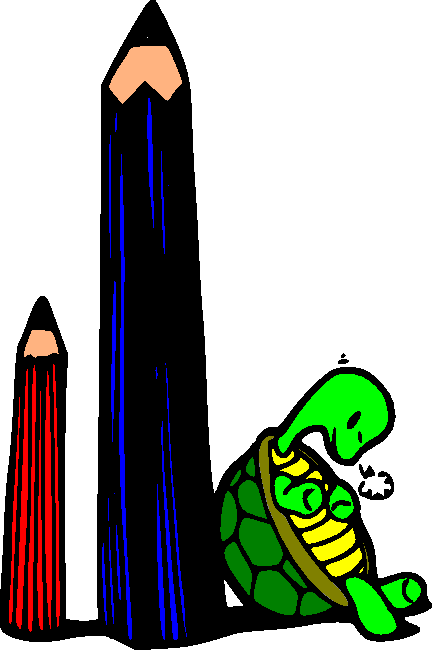
\includegraphics[scale=1]{images/tortue}
\end{center}

Même quand une tortue va à la vitesse maximale, elle continue de ne pas aller très vite.
Pour les tortues ce n'est pas vraiment un problème ---~elles ont du temps à perdre~--- mais quand on parle de graphiques sur un ordinateur, c'est un problème. Si vous avez une Nintendo DS, une PSP ou si vous jouez à des 
jeux sur votre ordinateur, pensez un moment aux graphiques que vous voyez affichés sur l'écran. Il y a différentes
manières de représenter des graphiques dans un jeu. Il y a les jeux en deux dimensions (2D) où les images sont «~plates~» et dans lesquels les personnages se déplacent verticalement et horizontalement mais pas en profondeur.
Ces jeux sont courrants sur les consoles mobiles et les téléphones mobiles. Et il y a des jeux en trois dimensions (3D) dans lesquelles les images ressemblent à la réalité et qui ajoutent de la «~profondeur~».

Tous ces types d'affichage graphiques ont une chose en commun ---~le besoin de dessiner sur l'écran vraiment rapidement. Avez-vous déjà essayé de faire vos propre animations? Celles où vous prenez un bloc de papier vierge et où dans le coin de la première page vous dessinez quelque chose (peut-être un bonhomme fil de fer) puis dans le coin de de la page suivante vous dessinez le même bonhomme avec une jambe qui a légèrement bougé. Puis sur la page d'après vous dessinez le même bonhomme avec la jambe un peu plus bougée encore. Et ainsi de suite sur toutes les pages du bloc. Quand vous avez fini, si vous faites deffiler les pages assez vite, il semblera que le bonhomme bouge. Ce sont les bases de la méthode utilisée pour toutes les animations sont faites, que vous regardiez un dessin animé ou un jeu vidéo sur une console ou un ordinateur. Vous dessinez quelque chose puis vous le dessinez à nouveau légèrement modifié pour donner l'illusion du mouvement. C'est pourquoi une tortue n'est pas bonne pour faire la plupart des graphiques. De manière à faire apparaître des images comme une image qui bouge, vous avez à dessiner chaque image de l'animation très vite.

Les graphiques en trois dimensions sont faits très différement des graphiques en deux dimensions, mais là aussi, l'idée-force est la même. Le temps que votre tortue ai fini de tracer une petite partie de l'image, il serait temps de tourner la page est de commencer à dessiner la suivante...



\section{Tortue de course}
Chaque language de programmation a des méthodes différentes pour dessiner sur un écran. Certaines méthodes sont rapides et d'autres sont lentes, ce qui veut dire que les programmeurs qui développent des vrais jeux 
doivent être vraiment attentif au language qu'ils choisissent pour travailler. Néanmoins, la plupart des graphiques de jeux sont fait avec des bibliothèques (des sortes de super modules) qui sont utilisables de manière similaire avec plusieurs langages de programmation.

Python a aussi différentes manière de faire des graphiques (incluant «~\texttt{turle}~»  que nous avons déjà utilisé) mais les meilleurs méthodes (d'un point de vue graphique) sont dans des modules et des bibliothèques qui ne sont pas inclues dans Python lui même (ni dans aucun autre langage).
Vous passerez probablement quelques années (ou mois pour les plus motivés) à programmer avant de comprendre comment installer et utiliser une de ces bibliothèques complexes.

Heureusement, il y a un module qui est fourni avec Python que nous pouvons utiliser pour faire des graphiques simples (à une vitesse plus rapide qu'une tortue). Peut-être assez rapide pour être appelé la «~tortue de course~» .
\begin{center}
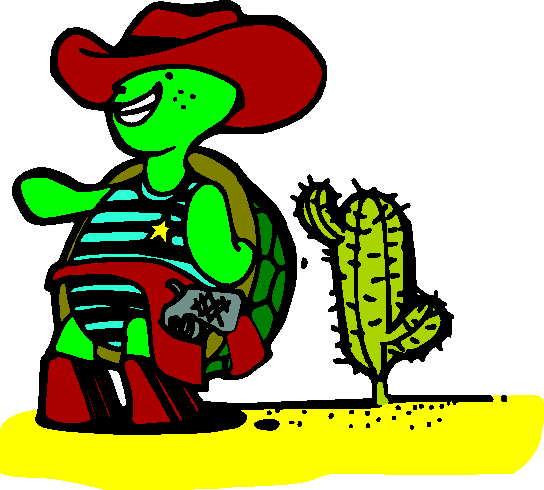
\includegraphics[scale=1]{images/tortue_rapide}
\end{center}

Ce module est appelé «~\texttt{tkinter}~» pour \emph{tool kit interface}, c'est à dire boîte à outils d'interface.
Si vous avez regardé  attentivement l'icone en haut à gauche des fenètre d'IDLE et de «~\texttt{turtle}~» vous avez pu voir 
\includegraphics[scale=1]{images/tk} pour \emph{tool kit}. Tkinter peut être utilisé pour faire de vraies applications comme IDLE (vous pourriez même créer un traitement de texte si vous le vouliez). Il peut aussi être utilisé pour faire de simples dessin. Nous pouvons créer une simple application avec un bouton avec le code suivant:

\begin{Verbatim}[frame=single,rulecolor=\color{mbleu}, label=à taper et sauver dans un nouveau fichier .py]
import tkinter
racine = tkinter.Tk()
racine.mainloop()
\end{Verbatim}

À la première ligne nous importons le contenu du module «~\texttt{tkinter}~» ainsi nous pouvons utiliser les fonctions de celui-ci. La plus utile «~\texttt{Tk()}~»  est utilisée à la deuxième ligne pour créer une fenètre vide dans laquelle nous pourrons ajouter des choses plus tard. Finalement à la troisième ligne nous utilisons la méthode «~\texttt{mainloop}~» (boucle principale) de notre fenètre vide «~\texttt{racine}~». Cette boucle principale est une boucle infinie que nous n'avons pas a gérer directement qui parcourt la fénètre et ces éléments pour voir si quelque chose à changé. Pour le moment notre application est vide, vous pouvez la fermer en utilisant le bouton de fermeture de fenètre de votre système d'exploitation qui devrait ressembler à  
\includegraphics[scale=1]{images/fermer} ou 
\includegraphics[scale=1]{images/fermer2}.

Nous allons maintenant ajouter un élément à notre application et pour commencer je vous propose un bouton:
\begin{Verbatim}[frame=single,rulecolor=\color{mbleu}, label=à taper et sauver dans un nouveau fichier .py]
import tkinter
racine = tkinter.Tk()
bouton = tkinter.Button(racine, text="Cliquez moi !")
bouton.pack()
racine.mainloop()
\end{Verbatim}

À la troisième ligne nous créons un nouveau bouton avec la commande «~\texttt{Button}~» de «~\texttt{tkinter}~» et nous lui attribuons le nom «~\texttt{bouton}~». Le boutton est créé en passant comme paramètre l'objet «~\texttt{racine}~»  que nous avions préalablement créé. Tous les petits «~machins\footnote{Il s'agit du terme québécois, le terme français est «~\texttt{composants d'interface graphique}~», généralement appelé composant ou  «~\texttt{widget}~»  de \emph{window gadget} (gadget de fénètre).}~» mis dans les fénètres doivent avoir un parent qui doit être passé en paramètre, ce parent est généralement une fenètre dans notre cas il s'agit de «~\texttt{racine}~». Le deuxième paramètre est un paramètre optionnel nommé qui indique quel texte mettre dans le bouton.

La quatrième ligne indique au bouton de se désiner lui-même. La commande «~\texttt{pack}~» indique au bouton comment il doit être «~tassé~»  dans la fenètre parente (ici «~\texttt{racine}~»). Sans paramètre la méthode utilisée de «~tasser~» les composants vers le haut (\emph{top}) par le bas. À ce point, la fenètre «~\texttt{racine}~» que nous avions créé se rétrécie elle-même à la taille de notre bouton qui contient les mots : «~Cliquez moi !~». Ce bouton ne fait pas grand chose (rien en fait) mais vous pouvez au moins cliquer dessus. 

\begin{center}

\fcolorbox{black}{lbleu}{
 \begin{minipage}{12cm}
\textbf{Paramètres nommés}\\

Ce n'est pas la première fois que nous utilisons des «~paramètres nommés~».
Ceux-ci fonctionnent comme les paramètres normaux mis à part qu'ils peuvent apparaître dans n'importe quel ordre, c'est pourquoi il faut fournir leur nom.

Par exemple, supposons que nous avons une fonction rectangle qui prend deux paramètres largeur et hauteur.
Normallement nous devons appeler cette fonction en utilisant quelque chose comme «~\texttt{rectangle(200,100}~» ce qui signifie que nous voulons dessiner un rectangle de 200 pixels de large par 100 pixels de haut. Mais que ce passerait-il si les paramètres pouvaient apparaitre dans n'importe quel ordre? Comment savoir ce qui est la largeur et ce qui est la hauteur? Dans ce cas il vaut mieux dire qui est qui, par exemple «~\texttt{rectangle(hauteur=100, largeur=200)}~». En réalité l'idée générale derrière les paramètres nommés est un peu plus compliquée que cela. Ils peuvent être utilisés diversement pour faire des fonctions plus flexibles ---~mais c'est un sujet pour un livre plus avancé que cette introduction à la programmation.
\end{minipage}
}
\end{center}


Nous pouvons changer notre exemple précédent un petit peu (n'oubliez de fermer la fenètre que nous venions de créer). Premièrerement nous allons créer une fonction pour afficher du texte, puis nous allons l'appeler quand nous cliquons sur le bouton.

\begin{Verbatim}[frame=single,rulecolor=\color{mbleu}, label=à taper]
import tkinter

def coucou() :
    print("coucou")

racine = tkinter.Tk()
bouton = tkinter.Button(racine, text="Cliquez moi !", command=coucou)
bouton.pack()

racine.mainloop()
\end{Verbatim}

Le paramètre «~\texttt{command}~» indique que nous voulons lancer une fonction à chaque fois que nous cliquons sur le bouton. Dans notre cas le paramètre «~\texttt{command}~» vaut «~\texttt{coucou}~», c'est à dire que la fonction «~\texttt{coucou}~» va être lancée à chaque clic. Au passage nous remarquons que Python lance considère tout élément (ici une fonction) comme un objet qui peut être manipulé. Si vous cliquez sur le bouton vous allez voir «~coucou~»  écrit sur la console à chaque fois que le bouton est cliqué.


La fenètre «~\texttt{racine}~» a une méthode «~\texttt{destroy}~» qui permet de détruire cette fenètre: il s'agit du \emph{destructeur} de l'objet). Elle peut être appelée de la même manière.

\begin{small}
\begin{Verbatim}[frame=single,rulecolor=\color{mbleu}, label=à taper]
import tkinter

def coucou() :
    print("coucou")

racine = tkinter.Tk()
bouton = tkinter.Button(racine, text="Cliquez moi !", command=coucou)
bouton.pack()

bouton_sortir = tkinter.Button(racine, text="Sortir", command=racine.destroy)
bouton_sortir.pack()

racine.mainloop()
\end{Verbatim}
\end{small}

Si vous cliquez sur le bouton «~\texttt{Sortir}~» l'application s'arrète.

Comme vous le voyez ci-dessu, j'ai été obligé de diminuer la taille mes caractères pour faire tenir la ligne de création du bouton. À ce propos Python ignore les identations à l'intérieur des parenthèses. Ce qui est utile même quand on n'est pas un livre. 

\begin{Verbatim}[frame=single,rulecolor=\color{gray}, label=ne pas saisir]
import tkinter

def coucou() :
    print("coucou")

racine = tkinter.Tk()
bouton = tkinter.Button(racine, text="Cliquez moi !", command=coucou)
bouton.pack()

bouton_sortir = tkinter.Button(racine, text="Sortir",
                               command=racine.destroy)
bouton_sortir.pack()

racine.mainloop()
\end{Verbatim}
 

\section{Dessins simples}

Les boutons ne sont pas vraiment utiles si vous voulez dessiner des choses sur l'écran. Ainsi nous avons besoins de créer et ajouter une sorte différente de composant: une zone de dessin appelé «~\texttt{Canvas}~» . Quand nous créons une zone de dessin nous avons besoin de passer en paramètres la hauteur et la largeur, contrairement au bouton qui prennait en paramètre un texte et une commande. Mis à part la hauteur (\emph{height}) et la largeur (\emph{width}) le code est similaire à celui utilisé pour le bouton.

\begin{Verbatim}[frame=single,rulecolor=\color{mbleu}, label=à taper]
import tkinter
racine = tkinter.Tk()

canvas = tkinter.Canvas(racine, width=500, height=500)
canvas.pack()

bouton_sortir = tkinter.Button(racine, text="Sortir",
                               command=racine.destroy)
bouton_sortir.pack()
racine.mainloop()
\end{Verbatim}

\begin{Verbatim}[frame=single,rulecolor=\color{mbleu}, label=à taper]
import tkinter
racine = tkinter.Tk()

canvas = tkinter.Canvas(racine, width=500, height=500)
canvas.pack()

bouton_sortir = tkinter.Button(racine, text="Sortir",
                               command=racine.destroy)
bouton_sortir.pack()
racine.mainloop()
\end{Verbatim}

Comme dans l'exemple du bouton, une fenètre racine est créée à la deuxième ligne. Quand vous «~tassez~»\footnote{Le verbe \emph{to pack} signifie emballer ou tasser} la zone de dessin «~\texttt{canvas}~» ligne cinq, la fénètre racine augmente de taille pour l'accueillir. Nous pouvons maintenant dessiner une ligne dans la zone de dessin en utilisant des coordonnées en pixels. Les coordonnées sont les positions des pixels dans la zone de dessin (verticalement et horizontalement). Dans une zone de dessin «~\texttt{tk}~»  les coordonnées décrivent à quelle distance nous sommes du coin en haut à gauche. Ces coordonnées sont données d'abord horizontalement de gauche vers la droite puis verticalement de haut en bas. L'ensemble des valeurs horizontales (de gauche vers la droite) est traditionnellement appelé axe des «~\emph{x}~». L'ensemble des valaures verticales (de haut en bas) est traditionnellement appelé axe des «~\emph{y}~». Le coin en haut à gauche, appelé l'origine, a pour coordonnées (0,0). Comme la zone de dessin fait 500 pixels de large et 500 pixel de haut le coin en bas à droite est situé aux coordonnées (499,499)\footnote{Ces valeurs sont théoriques, en pratique, en raison d'approximations faites par «~\texttt{tk}~», les valeurs effectives peuvent être légèrement différentes. Sur l'ordinateur du traducteur l'origine est située à (2,2) et le coin en bas à droite est à (501,501).}. Ainsi la ligne de la \autoref{fig:diag} peut être tracée en utilisant (0,0) pour coordonnées de départ et (499,499) pour coordonnées d'arrivée. Pour ce faire nous utilisons la méthode «~\texttt{create\_line}~»\footnote{Le verbe \emph{to create} signifie céer en anglais et \emph{line} signifie ligne.} du «~\texttt{Canvas}~» qui prend pour paramètre les coordonnées de points et les relie par des lignes. 
\begin{Verbatim}[frame=single,rulecolor=\color{mbleu}, label=à taper]
import tkinter
racine = tkinter.Tk()

canvas = tkinter.Canvas(racine, width=500, height=500)
canvas.pack()

bouton_sortir = tkinter.Button(racine, text="Sortir",
                               command=racine.destroy)
bouton_sortir.pack()
canvas.create_line(0,0, 499,499)

racine.mainloop()
\end{Verbatim}

\begin{figure}[h!]
\centering
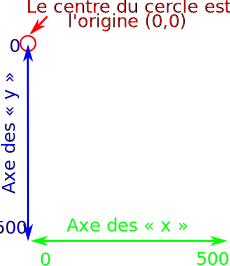
\includegraphics[scale=1]{images/diag}
\caption{Canvas (zone de dessin) avec les axes x et y}\label{fig:diag}
\end{figure}

Si vous avez du mal à lire les coordonnées, il convient de les séparer avec:
\begin{itemize}
\item des espace (comme ici);
\item ou un retour à la ligne.
\end{itemize}

\begin{Verbatim}[frame=single,rulecolor=\color{gray}, label=exemple]
canvas.create_line(  0,  0, 
                   499,499)
\end{Verbatim}

L'équivalent de:
\begin{Verbatim}[frame=single,rulecolor=\color{gray}, label=ne pas taper]
racine = tkinter.Tk()
canvas = tkinter.Canvas(racine, width=500, height=500)
canvas.pack()
canvas.create_line(0,0,499,499)
\end{Verbatim}
en «~\texttt{turtle}~» est: 
\begin{Verbatim}[frame=single,rulecolor=\color{gray}, label=ne pas taper]
turtle.setup(width=500, height=500)
tortue = turtle.Pen()
tortue.up()
tortue.goto(-250,250)
tortue.down()
tortue.goto(500,-500)
\end{Verbatim}

Pour faire la même chose (beaucoup plus lentement) le code est nettement plus long. Et encore nous avons utilisé la fonction «~\texttt{goto}~»\footnote{Le verbe \emph{to go} signifie aller et \emph{to} signifie «~à~».} donc je ne vous avais pas encore parlé\footnote{La méthode «~\texttt{goto}~» de «~\texttt{turtle}~» dit à la tortue de se déplacer par rapport à sa position actuelle d'un certain nombre de points horizontalement et verticalement.}. 

Avec «~\texttt{tkinter}~» le code est plus simple à comprendre et plus rapide. Il y a un grand nombre de méthodes disponibles avec l'objet «~\texttt{Canvas}~» dont certains qui ne nous seront pas très utiles, mais jetons un coup d'œil aux fonctions intéressantes.

\section{Dessiner des boîtes}

Dans «~\texttt{turtle}~», nous dessinons une boîte carrée en faisant: avancer, tourner, avancer, tourner, tourner, avancer, tourner, tourner, avancer et tourner. Éventuellement vous pouvez tracer un rectangle à la place d'un carré en changeant de combien vous avancez. Avec «~\texttt{tkinter}~» dessiner un carré ou un rectangle est considérablement plus simple ---~vous avez juste besoin de connaître les coordonnées des coins.
Dans un soucis de simpliffication et en raison de mon embompoint déjà trop important je rappelle ici pour une dernière fois les éléments qui seront à répéter tout le long de ce chapitre.

\begin{Verbatim}[frame=single,rulecolor=\color{mbleu}, label=à taper (ne sera plus indiqué par la suite)]
import tkinter
racine = tkinter.Tk()

canvas = tkinter.Canvas(racine, width=500, height=500)
canvas.pack()

bouton_sortir = tkinter.Button(racine, text="Sortir",
                               command=racine.destroy)
bouton_sortir.pack()
\end{Verbatim}

\begin{Verbatim}[frame=single,rulecolor=\color{mbleu}, label=à taper]
résultat=canvas.create_rectangle(50, 50, 
                                 10, 10)
print(résultat)
\end{Verbatim}

\begin{Verbatim}[frame=single,rulecolor=\color{mbleu}, label=à taper (ne sera plus indiqué par la suite)]
racine.mainloop()
\end{Verbatim}

La fonction «~\texttt{create\_rectangle}~» est utilisée pour créer des rectangles à partir des coordonnées de deux points. Les deux points sont les extrémités d'une diagonale. Le rectangle en question a des côtés horizontaux et verticaux.

Dans l'exemple ci-dessus nous dessinons un carré dont le premier coin (en bas à droite) est situé aux coordonnées (50,50) et dont le second coin (en haut à gauche) est situé aux coordonnées (10,10).
Vous vous demandez ce qu'est ce nombre que nous avons mis dans «~\texttt{résultat}~» puis que nous affiché dans le shell? C'est un numéro d'identification de la forme que nous venons de tracer (que cela soit une ligne, un rectangle ou un cercle). Nous reviendrons à ce numéro plus tard.

Les paramètres que nous avons passé pour créer le rectangle sont donc: la coordonnée horizontale \emph{x} du premier point, la coordonnée verticale \emph{y} du premier point, la coordonnée horizontale \emph{x} du second point, la coordonnée verticale \emph{y} du second point. On les appelle généralement \emph{x\textsubscript{1}}, \emph{y\textsubscript{1}}, \emph{x\textsubscript{2}} et \emph{y\textsubscript{2}}. Nous pouvons tracer un rectangle différent en choisissant \emph{x\textsubscript{2}} plus grand:

\begin{Verbatim}[frame=single,rulecolor=\color{mbleu}, label=à taper]
résultat=canvas.create_rectangle(50, 50, 
                                 100, 10)
print(résultat)
\end{Verbatim}

De même, nous pouvons changer ce rectangle en choisissant \emph{y\textsubscript{2}} encore plus grand:

\begin{Verbatim}[frame=single,rulecolor=\color{mbleu}, label=à taper]
résultat=canvas.create_rectangle(50, 50, 
                                 10, 200)
print(résultat)
\end{Verbatim}


Le dernier rectangle créé l'ai en disant simplement: place le premier coin 50 pixels sur la droite et 50 pixels vers le bas à partir de l'origine (le coin en haut à gauche); puis place un second coin 10 pixels vers la droite et 200 pixels vers le bas à partir de l'origine. À ce moment vous devriez avoir quelque chose comme sur la \autoref{fig:rectangle}.

\begin{figure}[h!]
\centering
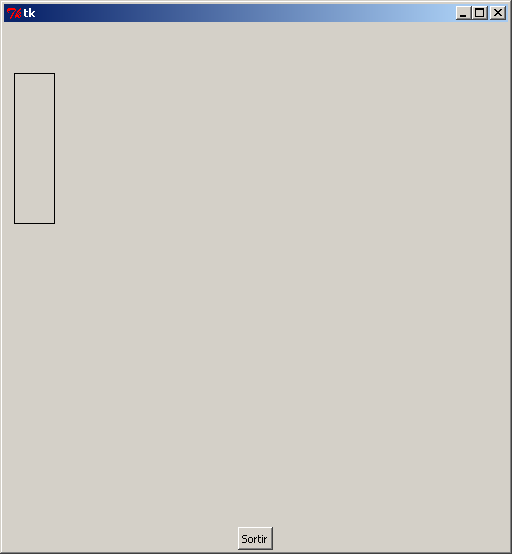
\includegraphics[scale=0.4]{images/rectangle}
\caption{Un rectangle réalisé avec «~\texttt{tk}~»}\label{fig:rectangle}
\end{figure}
 
Essayons de remplir le «~\texttt{Canvas}~» avec différentes tailles de rectangles. Nous pouvons pour cela utiliser un module appelé «~\texttt{random}~»\footnote{Le mot \emph{random} signifie élément aléatoire, c'est à dire dont on ne peut pas prédire la valeur. \emph{Random} vient du vieux français \emph{randir} qui signifie courrir.}. Premièrement nous allons importer le module en lançant: «~\texttt{import random}~». Pour la lisibilité du code il est conseillé de changer la première ligne de votre programme et d'y placer: «~\texttt{import tkinter, random}~».

Puis  nous pouvons créer une fonction en utilisant des nombres aléatoires pour les deux coins de chaque rectangle. La fonction à utiliser est appelé «~\texttt{randrange}~». La fonction «~\texttt{randrange}~» peut prendre pour paramètre un entier seulement (d'autres paramètres optionnels existent) et fournit alors un résultat entier aléatoire suppérieur ou égal à zéro et strictement inférieur au nombre rentré.

Nous pouvons une fonction pour créer des rectangles aléatoires:
\begin{Verbatim}[frame=single,rulecolor=\color{mbleu}, label=à taper]
def rectangle_aléatoire(largeur, hauteur):
    x1 = random.randrange(largeur)
    y1 = random.randrange(hauteur)
    x2 = random.randrange(largeur)
    y2 = random.randrange(hauteur)
    return canvas.create_rectangle(x1, y1, x2, y2)
\end{Verbatim}

Dans les deux premières lignes du corps de la fonction nous créons des variables pour le premier coin du rectangle en passant la largeur et la hauteur de la zone où nous allons dessiner nos rectangles. 
La fonction «~\texttt{randrange}~» avec un seul nombre en argument (pour plus de détail voir TOFIX) retourne un nombre aléatoire inférieur au nombre entré. Par exemple «~\texttt{randrange(10)}~» vous donnera un nombre entre 0 et 9 et «~\texttt{randrange(100)}~» vous donnera un nombre entre 0 et 99 et ainsi de suite. Les deux lignes suivantes crée les coordonnées pour le deuxième point. Puis nous créons le rectangle aléatoire avec ses variables. Ce rectangle aléatoire peut être un carré si \emph{x\textsubscript{1}+y\textsubscript{2}=y\textsubscript{1}+x\textsubscript{2}}, c'est à dire si les côtés sont égaux.

Nous pouvons utiliser notre fonction avec :
\begin{Verbatim}[frame=single,rulecolor=\color{mbleu}, label=à taper]
rectangle_aléatoire(500,500)
\end{Verbatim}

Nous pouvons aussi remplir le «~\texttt{Canvas}~» avec une centaine de rectangles aléatoires:
\begin{Verbatim}[frame=single,rulecolor=\color{mbleu}, label=à taper]
for x in range(0, 100):
    rectangle_aléatoire(500,500)
\end{Verbatim}

Au cas où vous vous seriez perdus votre programme complet doit donner:

\begin{Verbatim}[frame=single,rulecolor=\color{mbleu}, label=à taper]
import tkinter, random

racine = tkinter.Tk()
canvas = tkinter.Canvas(racine, width=500, height=500)
canvas.pack()
bouton_sortir = tkinter.Button(racine, text="Sortir",
                               command=racine.destroy)
bouton_sortir.pack()

def rectangle_aléatoire(largeur, hauteur):
    x1 = random.randrange(largeur)
    y1 = random.randrange(hauteur)
    x2 = random.randrange(largeur)
    y2 = random.randrange(hauteur)
    return canvas.create_rectangle(x1, y1, x2, y2)

for x in range(0, 100):
    rectangle_aléatoire(500,500)

racine.mainloop()
\end{Verbatim}

Et devrait produire quelque chose qui ressemble à la \autoref{fig:rectangles}.
\begin{figure}[h!]
\centering
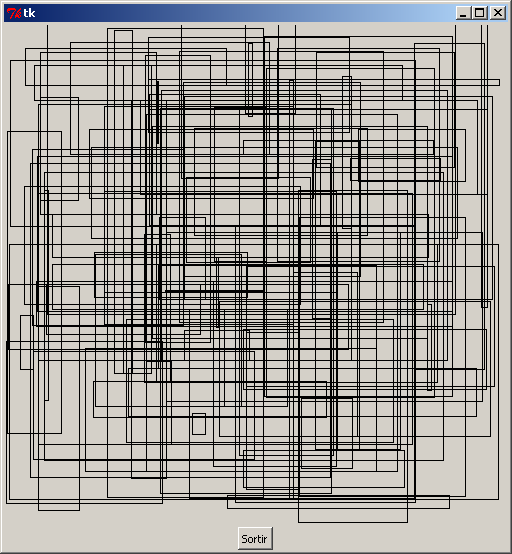
\includegraphics[scale=0.4]{images/rectangles}
\caption{Plein de rectangles}\label{fig:rectangles}
\end{figure}

C'est un peu le bazar mais c'est intéressant, néanmoins.
Notez au passage que chaque exécution du programme donne, très probablement, un résultat différent. Par conséquent votre résultat est sûrement différent du mien. Notez aussi comme l'affichage est rapide comparé à celui de «~\texttt{turtle}~».

Vous rappelez-vous que dans le chapitre présédent, nous avions modifié la couleur de la tortue avec des pourcentages des trois couleurs primaires: rouge, vert et bleu? Avec «~\texttt{tkinter}~» vous pouvez utiliser les couleur d'un manière similaire où d'une manière conçue initialement comme plus simple.

\subsubsection*{Commençons par la méthode faussement simple.}
La méthode «~\texttt{create\_rectangle}~» peut prendre un argument optionnel nommé «~\texttt{fill}~»\footnote{Le nom \emph{fill} signifie en anglais remplissage, du verbe «~\texttt{to fill}~» remplir.}. cet argument est une chaîne de caractères. Le nom des couleurs en anglais peut être en utilisé par exemple (\emph{red} signifie rouge):

\begin{Verbatim}[frame=single,rulecolor=\color{gray}, label=exemple]
canvas.create_rectangle(0, 0, 500, 500, fill='red')
\end{Verbatim}

Nous pouvons réfinir notre fonction «~\texttt{rectangle\_aléatoire}~»  de manière à disposer d'une paramètre optionnel pour le remplissage.

\begin{Verbatim}[frame=single,rulecolor=\color{mbleu}, label=à taper]
def rectangle_aléatoire(largeur, hauteur, remplissage=None):
    x1 = random.randrange(largeur)
    y1 = random.randrange(hauteur)
    x2 = random.randrange(largeur)
    y2 = random.randrange(hauteur)
    if remplissage==None:
        canvas.create_rectangle(x1, y1, x2, y2)
    else :	
        canvas.create_rectangle(x1, y1, x2, y2, fill=remplissage)
\end{Verbatim}

Nous pouvons alors créer une liste des couleurs en anglais\footnote{Les couleurs utilisées sont: noir, blanc, vert, rouge, bleu, orange, jaune, rose, une sorte de violet, une autre sorte de violet, magenta, cyan. Remarquez que \emph{purple} souvant traduit à tord pourpre et une sorte de violet en anglais.}. 

\begin{Verbatim}[frame=single,rulecolor=\color{mbleu}, label=à taper]
liste_couleur=['black', 'white', 'green',
               'red', 'blue', 'orange',
               'yellow', 'pink', 'purple',
               'violet', 'magenta', 'cyan']

for couleur in liste_couleur :
	rectangle_aléatoire(500,500,couleur)
\end{Verbatim}

Cette méthode a quatre inconvénients: 
\begin{itemize}
\item il faut connaître les noms des couleurs en anglais;
\item les noms des couleurs anglais ne correpondent pas forcément exactement aux même couleurs en français;
\item les couleurs nommées ne permettent pas de faire toutes les couleurs possibles;
\item les différents système d'exploitation (Linux, Mac Os X, Windows) n'ont pas tous les mêmes couleurs nommées (couleur différente voir absente ce qui crée une erreur).
\end{itemize}
\subsubsection*{Et maintenant la méthode faussement compliquée.}
Avec le module «~\texttt{turtle}~» nous avions fait de l'orangé avec 100\% de rouge, 85\% de vert et pas de bleu. Dans «~\texttt{tkinter}~» nous pouvons créer un rectangle orangé en utilisant

\begin{Verbatim}[frame=single,rulecolor=\color{mbleu}, label=à taper]
rectangle_aléatoire(500,500,'#ffd800')
\end{Verbatim}

La chaîne «~\texttt{\#ffd800}~» est en réalité une autre manière d'écrire des nombres.
Le format que nous utilisons courament est le format décimal: c'est à dire que nous utilisons dix chiffres: 0, 1, 2, 3, 4, 5, 6, 7, 8 et 9. Quand nous comptons nous commençons à 0 (en informatique en tout cas) et nous quand nous dépassons 9 nous utilisons deux chiffres 10 (1 puis 0).

Les ordinateurs sont beaucoup plus bêtes que nous et compte en réalité en binaire: ils utilisent deux chiffres: 0 et 1. Quand ils dépassent 1 (si si!) ils utilissent deux chiffres 10 (1 puis 0). La suite des nombre en binaire donne: 0, 1, 10, 11, 100, 101, 111, 1000, 1001... Par exemple deux mille neuf s'écrit en binaire 11111011001 ce qui est un peu long. Cette utilisation du binaire provient du fait que les ordinateurs ont des mémoires qui sont soient soit remplies soit vide. Cet élément d'information s'appelle un «~bit~» (prononcé bite ☺).\\

\emph{Il existe d'ailleurs une blague: «~Il existe \emph{10} types de personnes dans le monde, ce qui comprennent le binaire et les autres~»\footnote{Le 10 étant à comprendre en binaire c'est à dire deux.}.}\\


Nos grand anciens ont donc décidé d'utiliser une notation plus pratique pour les humains mais simple à utiliser l'hexadécimal: c'est à dire que nous utiliserons seize chiffres: 0, 1, 2, 3, 4, 5, 6, 7, 8, 9, a, b, c, d, e et f. Quand nous comptons en hexadécimal nous commençons à zéro et quand nous dépassons f (quinze) nous utilisons deux chiffre 1 et 0. Généralement en informatique nous utilisons deux chiffres qui permettent de compter de zéro à deux cent cinquante cinq «~\texttt{ff}~» .
Cet élément élément d'information s'appelle un «~octet~» (prononcé octé). L'octet correspond à huit bits. C'est cette unité de mesure qui est utilisée sous la forme de kilooctet\footnote{Pour information il s'agit généralement de kibioctet, 2\up{10} octets c'est à dire 1024 octets.}, de mégaoctet\footnote{Souvent, il s'agit d'un mébioctet qui vaut 2\up{20} (1024\textsf{x}1024) octets.}, de gigaoctet\footnote{Souvent, il s'agit d'un gibioctet qui vaut 2\up{30} (1024\textsf{x}1024\textsf{x}1024) octets.} voir de teraoctet\footnote{Souvent, il s'agit d'un tébioctet qui vaut 2\up{40} (1024\textsf{x}1024\textsf{x}1024\textsf{x}1024) octets.}.

Revenons à notre couleur «~\texttt{\#ffd800}~» comment lit on cette valeur? En fait le \# est là pour indiquer qu'il s'aggit d'un nombre hexagonal puis viennent trois octets par couple de deux caractère: les deux premiers «~\texttt{ff}~» pour rouge, les deux suivant «~\texttt{d8}~» pour vert et les deux derniers «~\texttt{00}~» pour bleu. La valeur décimale se lit: seize fois le premier chiffre plus le second. Le nombre «~\texttt{ff}~» vaut seize fois quinze (f) plus quinze (deux cent cinquante cinq). Le nombre «~\texttt{d8}~» vaut seize fois treize  «~\texttt{d}~» plus huit (deux cent seize). Inversement nous pouvons définir une fonction pour traduire les pourcentages de couleurs dans les valeurs utilisables par «~\texttt{create\_rectangle}~».

\begin{Verbatim}[frame=single,rulecolor=\color{mbleu}, label=à taper]
def couleurshex(rouge, vert, bleu):
    rouge = 255*(rouge/100.0)
    vert = 255*(vert/100.0)
    bleu = 255*(bleu/100.0)
    return '#%02x%02x%02x' % (rouge, vert, bleu)
\end{Verbatim}

Si nous appelons la fonction «~\texttt{couleurshex}~» avec 100 pour le rouge, 85 pour le vert et 0 pour le bleu nous donne dans le shell «~\texttt{\#ffd800}~».

\begin{Verbatim}[frame=single,rulecolor=\color{mbleu}, label=à taper]
print(couleurshex(100,85,0))
\end{Verbatim}

Nous pourrions écrire le code suivant pour créer un ractangle orangé.

\begin{Verbatim}[frame=single,rulecolor=\color{gray}, label=exemple]
rectangle_aléatoire(500,500,couleurshex(100,85,0))
\end{Verbatim}

Nous pouvons créer une couleur violet vif  en utilisant 98\% de rouge, 1\% de vert et 77\% de bleu:
\begin{Verbatim}[frame=single,rulecolor=\color{gray}, label=exemple]
rectangle_aléatoire(500,500,couleurshex(98,1,77))
\end{Verbatim}

Nous pouvons aussi créer une fonction «~\texttt{couleur\_surprise}~».
\begin{Verbatim}[frame=single,rulecolor=\color{mbleu}, label=à taper]
def couleur_surprise():
    return '#%02x%02x%02x' %(random.randrange(256),
                       random.randrange(256),
                       random.randrange(256))
\end{Verbatim}
 
Puis nous pouvons nous en servir avec «~\texttt{rectangle\_aléatoire}~». Pour information voila ce à quoi votre code doit ressembler.

\begin{Verbatim}[frame=single,rulecolor=\color{mbleu}, label=à taper]
import tkinter, random

racine = tkinter.Tk()
canvas = tkinter.Canvas(racine, width=500, height=500)
canvas.pack()
bouton_sortir = tkinter.Button(racine, text="Sortir",
                               command=racine.destroy)
bouton_sortir.pack()

def rectangle_aléatoire(largeur, hauteur, remplissage=None):
    x1 = random.randrange(largeur)
    y1 = random.randrange(hauteur)
    x2 = random.randrange(largeur)
    y2 = random.randrange(hauteur)
    if remplissage==None:
        canvas.create_rectangle(x1, y1, x2, y2)
    else :	
        canvas.create_rectangle(x1, y1, x2, y2, fill=remplissage)

def couleur_surprise():
    return couleurshex(randrange(256),randrange(256),randrange(256))


for x in range(0, 100):
    rectangle_aléatoire(500,500, couleur_surprise())

racine.mainloop()
\end{Verbatim}

Vous obtenez alors un résultat similaire à celui de la \autoref{fig:rects}. Ce programme vaut peut-être la peine d'être mis sur le bureau avec l'extension«~\texttt{.pyw}~» pour le monter à d'autres personnes?
\begin{figure}[h!]
\centering
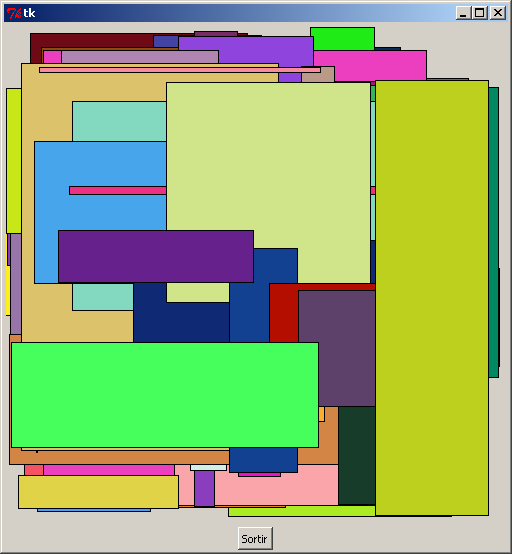
\includegraphics[scale=0.4]{images/rectangles2}
\caption{Rectangles colorés aléatoires}\label{fig:rects}
\end{figure}

\section{Dessiner des ovales}
Comme nous avons dessiné des rectangles, nous pouvons dessiner des ovales comme vous pouvez le voir sur la \autoref{fig:ovalebis}.

\begin{Verbatim}[frame=single,rulecolor=\color{mbleu}, label=à taper]
canvas.create_oval(5, 5, 300, 200)
\end{Verbatim}

\begin{figure}[h!]
\centering
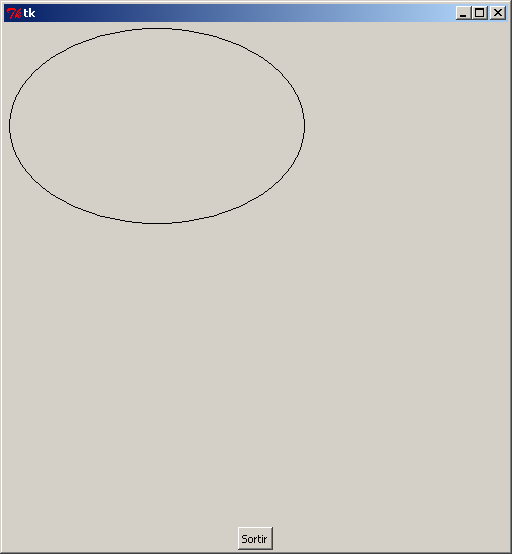
\includegraphics[scale=0.4]{images/ovalebis}
\caption{Un ovale}\label{fig:ovalebis}
\end{figure}

L'ovale est créé avec la fonction «~\texttt{create\_oval}~» inscrit dans un rectangle imaginaire décrit par les points (5,5) et (300,200). Dessinons un rectangle pour mieux comprendre cette explication.

\begin{Verbatim}[frame=single,rulecolor=\color{mbleu}, label=à taper]
canvas.create_rectangle(5, 5, 300, 200, outline="#ff0000")
canvas.create_oval(5, 5, 300, 200)
\end{Verbatim}

Le paramètre «~\texttt{outline}~» (bordure) permet d'indiquer la couleur du bord d'un rectangle ou d'un ovale.
Ici «~\texttt{\#ff0000}~» permet de dessiner un rectangle rouge. Vous pouvez le voir sur la \autoref{fig:ovale}.

\begin{figure}[h!]
\centering
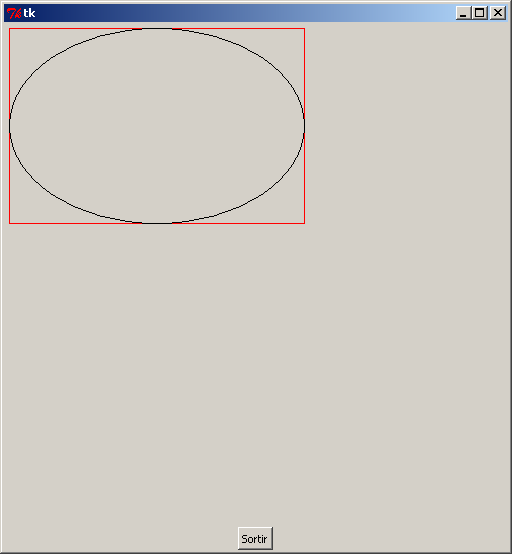
\includegraphics[scale=0.4]{images/ovale}
\caption{Un ovale inscrit dans un rectangle}\label{fig:ovale}
\end{figure}

Cet exemple dessine d'abord un rectangle entre (5,5) et (300,200) puis un oval dans qui est inscrit dans un rectangle défini par les coins (5,5) et (300,200). La fonction «~\texttt{create\_oval}~» donnera exactement le même résultat sans avoir dessiner le rectangle auparavent.

En langage mathématique les ovales que nous dessinons s'appellent des élipses.
S'il est possible avec la commande «~\texttt{create\_oval}~»  des élipses, il existe un type d'élipse particulier que vous connaissez bien: le cercle!  Si le rectangle imaginaire dans lequel nous dessinons l'élipse est un carré, le résultat est un cercle comme vous pouvez le voir sur la \autoref{fig:cerclebis}.

\begin{Verbatim}[frame=single,rulecolor=\color{mbleu}, label=à taper]
canvas.create_oval(5, 5, 300, 300)
\end{Verbatim}

\section{Dessiner des arcs}
Un arc de cercle est un boût de cercle. Dans «~\texttt{tkinter}~» nous pouvons dessiner des arcs de cercle ou d'élipse. Pour rappel, une élipse est une sorte de cercle applati. 
Les arcs sont définis comme des portions d'ovale eux même décrits à partir de deux points comme à la section précédente.

\begin{Verbatim}[frame=single,rulecolor=\color{mbleu}, label=à taper]
canvas.create_arc(10, 10, 200, 100, extent=180, style='arc')
\end{Verbatim}



Cette commande crée un rectangle virtuel (qui n'existe pas) trace virtuellement une élipse puis prend un bout de celle-ci.
De la même manière que pour les cercles de «~\texttt{turtle}~» le paramètre «~\texttt{extent}~» indique l'extension de l'arc. Le style «~\texttt{'arc'}~» indique quels sont les bords à tracer. Deux autres styles sont disponibles le mode par défaut «~\texttt{'pieslice'}~»\footnote{Le mot \emph{pie slice} signifie part (pour \emph{slice}) de tarte (pour \emph{pie}).}qui trace les rayons depuis le centre du cercle ou de l'élipse, et le style «~\texttt{'chord'}~»\footnote{Le nom \emph{chord} signifie corde en anglais} trace l'arc et la ligne entre les deux extrémités de l'arc.

Nous pouvons matérialiser cette construction avec le code suivant.

\begin{Verbatim}[frame=single,rulecolor=\color{mbleu}, label=à taper]
canvas.create_rectangle(10, 10, 400, 300, outline="#ff0000")
canvas.create_arc(10, 10, 400, 300, extent=180, style='arc')
\end{Verbatim}

Vous pouvez voir le résultat sur la \autoref{fig:arc}.
\begin{figure}[h!]
\centering
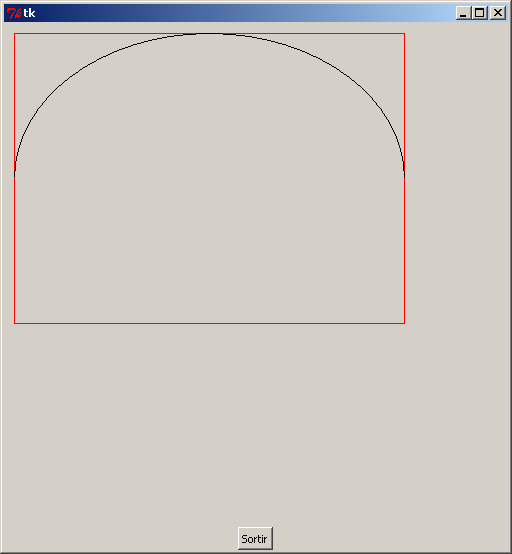
\includegraphics[scale=0.4]{images/arc}
\caption{Arc inscrit dans un rectangle}\label{fig:arc}
\end{figure}

Si vous ne savez pas encore ce que sont les degrés rappelez vous le cercle des degrés de la \autoref{fig:degres} page \autoref{fig:degres}. Si cela n'est pas clair rappelez vous que
\begin{itemize}
\item un arc de 90° est un arc d'un quart de tour;
\item un arc de 180° est un arc d'un demi tour;
\item un arc de 359° est un arc de presqu'un tour complet.
\end{itemize}

Pour note: 360° sont en fait égaux à 0°, malheureusement quelques fois pour nous «~\texttt{tkinker}~» sait cela et ne dessinera rien si vous rentrez 360° ou 0°. Voici quelques lignes de code pour montrer quelques arcs descendant le long de la zone de dessin. Ainsi vous pouvez voir les différences entre différents angles d'arcs sur la \autoref{fig:arcs}
\begin{Verbatim}[frame=single,rulecolor=\color{mbleu}, label=à taper]
canvas.create_arc(10, 10, 200, 100, extent=45, style='arc')
canvas.create_arc(10, 80, 200, 160, extent=90, style='arc')
canvas.create_arc(10, 160, 200, 240, extent=135, style='arc')
canvas.create_arc(10, 240, 200, 320, extent=180, style='arc')
canvas.create_arc(10, 320, 200, 400, extent=359, style='arc')
\end{Verbatim}

\begin{figure}[h!]
\centering
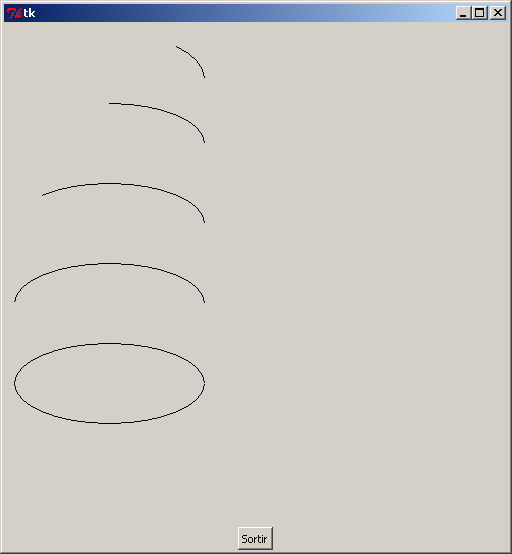
\includegraphics[scale=0.4]{images/arcs}
\caption{Différents arcs}\label{fig:arcs}
\end{figure}


\section{Dessiner des polygones}
Un polygone est une figure avec trois côtés ou plus. 
Les triangles, les carrés, les rectangles, les pentagones, les hexagones et de nombreux autres sont tous des exemples de polygones. Les polygones peuvent être réguliers, avec des angles égaux de des cotés égaux, ou irréguliers. 

La fonction «~\texttt{create\_polygon}~» permet de créer des polygones à partir des coordonnées de sommets.
Par exemple, pour tracer un triangle, vous avez besoin de fournir trois couples de coordonnées (un couple pour chaque commet). Voici un petit exemple que vous pouvez voir sur la \autoref{fig:triangle}.

\begin{Verbatim}[frame=single,rulecolor=\color{mbleu}, label=à taper ne sera pas répété]
import tkinter, random

racine = tkinter.Tk()
canvas = tkinter.Canvas(racine, width=500, height=500)
canvas.pack()
bouton_sortir = tkinter.Button(racine, text="Sortir",
                               command=racine.destroy)
bouton_sortir.pack()
\end{Verbatim}
\begin{Verbatim}[frame=single,rulecolor=\color{mbleu}, label=à taper]
canvas.create_polygon(10, 10, 100, 10, 100, 50)
\end{Verbatim}
\begin{Verbatim}[frame=single,rulecolor=\color{mbleu}, label=à taper ne sera pas répété]
racine.mainloop()
\end{Verbatim}

\begin{figure}[h!]
\centering
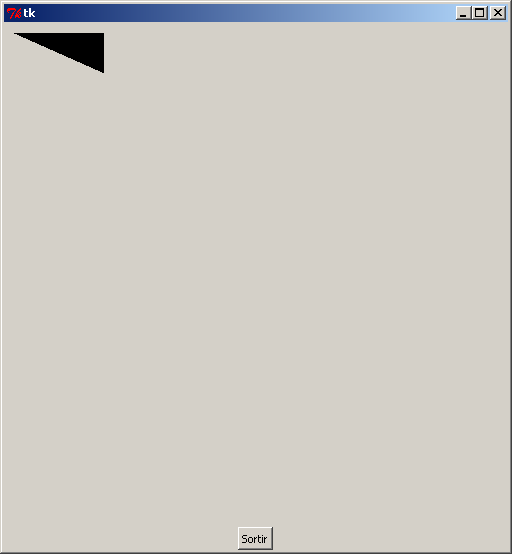
\includegraphics[scale=0.4]{images/triangle}
\caption{Un triangle plein}\label{fig:triangle}
\end{figure}

Comme on le voit les polygones sont pas défaut remplis de noir. Le paramètre nommé «~\texttt{fill}~» permet de choisir le remplissage. Si l'on fixe ce paramètre à une chaîne vide «~\texttt{""}~», il n'y aura pas de remplissage.

\begin{Verbatim}[frame=single,rulecolor=\color{mbleu}, label=à taper]
canvas.create_polygon(10, 10, 100, 10, 100, 50, fill="")
\end{Verbatim}

Cette fonction ne donne aucun résultat. En effet les polygonnes sont rempliset sans bordure par défaut. Il convient donc de fixer une couleur de la bordure avec «~\texttt{outline}~».

\begin{Verbatim}[frame=single,rulecolor=\color{mbleu}, label=à taper]
canvas.create_polygon(10, 10, 100, 10, 100, 50, 
                      fill="", outline="#000000")
\end{Verbatim}

Nous pouvons aussi dessiner un autre polygone irrégulier et un polygone régulier.

\begin{Verbatim}[frame=single,rulecolor=\color{mbleu}, label=à taper]
canvas.create_polygon(10, 10, 100, 10, 100, 50,
                      fill="", outline="#000000")
canvas.create_polygon(200, 10, 240, 30,
                      120, 100, 140, 120,
                      fill="", outline="black")
canvas.create_polygon(260, 10, 500, 10,
                      500, 260, 260, 260,
                      fill="#00ff00", outline="black")
\end{Verbatim}

Vous pouvez voir le résultat sur la figure \autoref{fig:polys}.
\begin{figure}[h!]
\centering
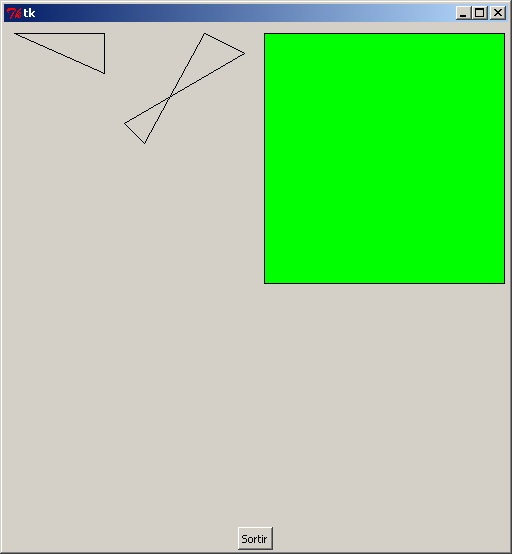
\includegraphics[scale=0.4]{images/polys}
\caption{Divers polygones}\label{fig:polys}
\end{figure}

\section{Dessiner des images}
\label{sec:dessinimages}

Nous avons besoin en premier lieu d'une image préxistante, Puis nous utiliserons la méthode «~\texttt{image}~» de l'objet «~\texttt{canvas}~». Cela semble un peu illogique, mais cela fonctionnne comme suit: 
Pour pouvoir manipuler une image, vous devez savoir où elle est pour pouvoir y accéder avec Python. Je vous propose de créer une image «~\texttt{test.gif}~» sur le bureau. En effet, Python (pour être exact tkinter) peut par défaut utiliser des images aux formats «~\texttt{gif}~», «~\texttt{pgm~}~» et «~\texttt{ppm}~»\footnote{La bibliothèque «~\texttt{PIL}~», c'est à dire \emph{Python imaging library,} peut être utilisée pour manipuler d'autres formats d'image.}.



\begin{Verbatim}[frame=single,rulecolor=\color{mbleu}, label=à taper]
import tkinter

racine = tkinter.Tk()
canvas = tkinter.Canvas(racine, width=500, height=500)
canvas.pack()
bouton_sortir = tkinter.Button(racine, text="Sortir",
                               command=racine.destroy)
bouton_sortir.pack()


import os,platform

def chemin_bureau() :
    if platform.release()=='XP' :
        return os.path.join(os.environ['HOME'],"Bureau")
    else :
        return os.path.join(os.environ['HOME'],"Desktop")
    
cheminfichier = os.path.join(chemin_bureau(),'test.gif')

monimage = tkinter.PhotoImage(file=cheminfichier)
canvas.create_image(0, 0, image=monimage, anchor=tkinter.NW)

racine.mainloop()
\end{Verbatim}

Dans les premières lignes nous inialisons une fenètre et une zone de dessin comme précédemment.
Puis l'image «~\texttt{monimage}~» est chargée à partir du fichier «~\texttt{test.gif}~» en utilisant la fontion «~\texttt{tkinter.Photoimage}~».

Nous utilisons ensuite la méthode «~\texttt{canvas.create\_image}~» de notre zone de dessin pour afficher notre image. Vous devriez voir apparaître quelque chose qui ressemble à la \autoref{fig:gif}. Comme indiqué précédement PhotoImage peut traiter des fichiers d'images avec aux formats «~\texttt{gif}~», «~\texttt{pgm~}~» et «~\texttt{ppm}~».
Il y a de nombreux types d'images différents qui peuvent être créés comme par exemple les images «~\texttt{jpeg}~» qui sont stockées par les appareils photos avec l'extension «~\texttt{.jpg}~». 
La bibliothèque de traitement d'image de Python (\emph{Python imaging library} ajoute la possibilité de traiter de charger la plupart des types d'images ainsi qui certaines méthodes de traitement comme aggrandir ou réduire, changer les couleurs ou tourner les images.  Néanmoins, installer et utiliser la bibliothèque de traitement d'image de Python et légèrement en dehors du sujet de ce livre\footnote{La  bibliothèque de traitement d'image de Python peut être trouvée à l'adresse \url{http://www.pythonware.com/products/pil/index.htm}. Malheureusement à la date d'écriture de ce livre (23 juillet 2009) le portage vers Python~3 n'a pas encore été achevé.}. 

Notez que vous pouvez utiliser la fonction «~\texttt{os.getcwd()}~» pour connaître le répertoire courant utilisé par Python. Dans une ligne de commande ou un \emph{shell} Python vous pouvez taper les commandes suivantes.
\begin{Verbatim}[frame=single,rulecolor=\color{mbleu}, label=à taper]
>>> import os 
>>> print(os.getcwd())
C:\Python30
\end{Verbatim}

Il en résultera probablement quelque chose comme le chemin indiqué à la dernière ligne. Vous pouvez copier des ressources (comme les images) auquelles vos programmes accèdent très souvent dans ce répertoire. Vous pourriez par exemple y copier l'image «~\texttt{test.gif}~» et la charger avec la commande «~\texttt{monimage = tkinter.PhotoImage(file=testk.gif)}~».

\section{Aminimations simples}
Jusqu'à mainteant nous avons dessiné des images qui ne bougeaient pas. Quand est-il des animations?
Les animations ne sont pas forcément le point fort de Tk, mais je peux vous y initier.\\

\emph{Les animations ne sont d'ailleurs pas non plus le point fort des livres!}\\

Par exemple nous pouvons créer un triangle puis le faire bouger à travers l'écran avec le code suivant:
\begin{Verbatim}[frame=single,rulecolor=\color{mbleu}, label=à taper]
import tkinter

racine = tkinter.Tk()
canvas = tkinter.Canvas(racine, width=500, height=500)
canvas.pack()
bouton_sortir = tkinter.Button(racine, text="Sortir",
                               command=racine.destroy)
bouton_sortir.pack()


import time

numéro_forme=canvas.create_polygon(10, 10, 10, 60, 50, 35)
for x in range(0, 100):
    canvas.move(numéro_forme, 5, 0)
    racine.update()
    time.sleep(0.05)

racine.mainloop()
\end{Verbatim}

Juste après avoir lancé le programme un triangle va commencer à se déplacer (vous pouvez le voir à mi-chemin sur la \autoref{fig:triangle}. Comment cela fonctionne-t-il?

Après une initialisation nous dessinons un triangle avec «~\texttt{canvas.create\_polygon}~». 
Nous stockons le numéro de la forme retourné par «~\texttt{canvas.create\_polygon}~» dans la variable «~\texttt{numéro\_forme}~», pour information il s'agit de la forme numéro un.
Puis nous initialison un itérateur qui va prendre les valeurs de un à quatre-vingt dix-neuf. Le bloc utilisé juste après est le code pour bouger le triangle lentement. Tout d'abord la méthode «~\texttt{canvas.move}~»\footnote{Le mot «\emph{move}» signifie bouger en anglais de mouvoir.}  prend trois argument le numéro d'un élément à bouger, le nombre de points horizontaux vers la droite pour le déplacement (un nombre négatif crée un déplacement vers la gauche) et le nombre de points verticaux vers le bas (un nombre négatif crée un déplacement vers le haut). Dans notre exemple le triangle (objet un) est déplacé à chaque pas de cinq points vers la droite à chaque pas de l'itérateur.  
Puis nous utilisons la méthode «~\texttt{racine.update}~» pour obliger l'objet racine à se mettre à jour (\emph{update}). Si nous n'indiquons pas cela tkinter attendrait jusqu'à la fin de la boucle avant de bouger le triangle à sa position finale.  Enfin, nous disons à Python d'attendre cinq centièmes de seconde avec la méthode «~\texttt{time.sleep}~» du module «~\texttt{time}~»\footnote{Le mot \emph{sleep} signifie dormir et le mot \emph{time} signifie temps.}.

Nous pouvons si nous le souhaitons ajouter une deuxième boucle en utilisant  «~canvas.move(numéro\_forme, -5, 0)~»  pour ramener le triangle à sa position initiale.


Nous pouvons aussi déplacer le triangle en diagonale par exemple.

\begin{Verbatim}[frame=single,rulecolor=\color{mbleu}, label=à taper]
import tkinter

racine = tkinter.Tk()
canvas = tkinter.Canvas(racine, width=500, height=500)
canvas.pack()
bouton_sortir = tkinter.Button(racine, text="Sortir",
                               command=racine.destroy)
bouton_sortir.pack()


import time

numéro_forme=canvas.create_polygon(10, 10, 10, 60, 50, 35)
for x in range(0, 100):
    canvas.move(numéro_forme, 5, 5)
    racine.update()
    time.sleep(0.05)
for x in range(0, 100):
    canvas.move(numéro_forme, -5, -5)
    racine.update()
    time.sleep(0.05)


racine.mainloop()
\end{Verbatim}

\section{Réagir aux événements}
Nous pouvons aussi faire réagir le triangle quand quelqu'un presse une touche en liant une action à un événement. Les événements sont des choses qui arrivent pendant que le programme fonctionne et qu'il peut traiter comme le fait que quelqu'un presse une touche, actionne un bouton ou même ferme une fenètre. Vous pouvez configurer Tk pour surveiller ces événements et faire quelque chose en réaction. Pour commencer à gérer les événements nous avons besoin de commencer par créer une fonction. Supposons que nous voulons que le triangle bouge vers le bas quand la touche entrée est préssée. Nous pouvons définir une fonction pour déplacer le triangle.
\begin{Verbatim}[frame=single,rulecolor=\color{gray}, label=ne pas taper]
def déplacertriangle(event):
    canvas.move(1, 5, 0)
\end{Verbatim}


Figure 9.14: The triangle moving down the screen.


La fonction «~\texttt{déplacerobjet}~» doit avoir un seul paramètre «~\texttt{event}~» (événement en anglais) pour réaggir à un événement. Ainsi nous disons à Python que cette fonction doit être utilisé pour être lié à un événement.


\begin{Verbatim}[frame=single,rulecolor=\color{mbleu}, label=à taper]
import tkinter

racine = tkinter.Tk()
canvas = tkinter.Canvas(racine, width=500, height=500)
canvas.pack()
bouton_sortir = tkinter.Button(racine, text="Sortir",
                               command=racine.destroy)
bouton_sortir.pack()


import time

numéro_forme=canvas.create_polygon(10, 10, 10, 60, 50, 35)
numéro_figure=canvas.create_polygon(110, 110, 110, 160, 150, 135)

def déplaceobjet(event):
    canvas.move(numéro_figure, 0, 3)

canvas.bind_all('<KeyPress-Return>', déplaceobjet)

racine.mainloop()
\end{Verbatim}

Le premier paramètre de la méthode «~\texttt{canvas.bind\_all}~» (\emph{bind:} lier, \emph{all:} tout) quel est l'événement que nous voulons voir surveiller par Tk. Dans ce cas précis, il s'agit de l'événement «~\texttt{KeyPress-Return}~» qui à lieu lorsqu'on presse la touche (\emph{key}) entrée (\emph{return}). Le deuxième argument à Tk quelle fonction est associée à cet événement; ici nous utilisons la fonction  «~\texttt{déplaceobjet}~». Nous disons à Tk quelle fonction lancer quand la touche entrée est pressée. Lancez ce code, contrôlez que la fenêtre crée est sélectionnée et appuyez sur entrée.

Attelons nous maintenant à changer la direction de déplacement du triangle. Tout d'abord changeons la fonction déplacerobjet de manière à ce quelle réagisse différemment selon la touche appuyée.
\begin{Verbatim}[frame=single,rulecolor=\color{mbleu}, label=à taper]
def déplaceobjet(event):
    if event.keysym == 'Up':
        canvas.move(numéro_figure, 0, -3)
    elif event.keysym == 'Down':
        canvas.move(numéro_figure, 0, 3)
    elif event.keysym == 'Left':
        canvas.move(numéro_figure, -3, 0)
    else:
        canvas.move(numéro_figure, 3, 0)
\end{Verbatim}

L'objet «~\texttt{event}~» qui est passé à déplaceobjet contient de nombreuses attributs\footnote{Les attributs sont des valeurs nommées qui décrivent quelque chose de l'objet. Par exemple, un attribut du ciel est sa couleur qui est bleu quelque fois, un attribut d'une voiture est sont nombre de places. En programmation, un attribut a un nom et une valeur.}. Un de ces attribut est «~\texttt{keysym}~» qui est une chaîne qui contient le nom de la touche appuyée en anglais. Si «~\texttt{keysym}~» contient la chaîne «~\texttt{Up}~», nous appelons «~\texttt{canvas.move}~»  avec les paramètres «~\texttt{(numéro\_figure, 0, -3)}~» de manière à déplacer la forme identifiée par son numéro de zéro pixels vers la droite et de moins trois pixels vers le bas c'est à dire de trois pixels vers le haut. Si la chaîne est «~\texttt{Down}~» nous déplaçons l'objet vers le bas, si c'est «~\texttt{Left}~» vers la gauche et sinon vers la droite. Notez que nous aurions pu choisir de déplacer l'objet vers la droite seulement quand la touche droite «~\texttt{Right}~» est pressée.

\begin{Verbatim}[frame=single,rulecolor=\color{mbleu}, label=à taper]
import tkinter
racine = tkinter.Tk()
canvas = tkinter.Canvas(racine, width=800, height=500)
canvas.pack()


numéro_figure=canvas.create_polygon(110, 110, 110, 160, 150, 135)


def déplaceobjet(event):
    if event.keysym == 'Up':
        canvas.move(numéro_figure, 0, -3)
    elif event.keysym == 'Down':
        canvas.move(numéro_figure, 0, 3)
    elif event.keysym == 'Left':
        canvas.move(numéro_figure, -3, 0)
    else:
        canvas.move(numéro_figure, 3, 0)

canvas.bind_all('<KeyPress>', déplaceobjet)

racine.mainloop()
\end{Verbatim}

Avec cet exemple le triangle se déplace maintenant dans la direction de la flèche que vous pressez ou vers la droite pour toutes les touches.
